\subsection*{Problema 04}

\textbf{Enunciado:}
Probar que para todo entero $n \ge 2$:
\begin{align*}
\sum_{k=2}^{n} \dfrac{1}{k} < \ln(n) < \sum_{k=1}^{n-1} \dfrac{1}{k}
\end{align*}

\textbf{Solución:}
La función $f(t) = \dfrac{1}{t}$ es continua y decreciente en el intervalo $[1, \infty)$. 
Sabemos que el logaritmo natural se define mediante la integral:
\begin{align*}
\ln(n) = \int_{1}^{n} \dfrac{1}{t} \, dt
\end{align*}

Podemos aproximar esta integral mediante sumas de Riemann usando una partición regular del intervalo $[1, n]$ con subintervalos de ancho $\Delta t = 1$, cuyos puntos extremos son $t_k = k$ para $k = 0, 1, 2, \dots, n$.

Para la cota inferior, consideramos los rectángulos inscritos (suma inferior) en cada subintervalo $[k, k+1]$ con altura dada por el extremo derecho $f(k+1) = \dfrac{1}{k+1}$:
\begin{align*}
\int_{1}^{n} \dfrac{1}{t} \, dt &> \sum_{k=1}^{n-1} f(k+1) \cdot \Delta t \\
\int_{1}^{n} \dfrac{1}{t} \, dt &> \sum_{k=1}^{n-1} \dfrac{1}{k+1}
\end{align*}

Cambiando el índice con $j = k+1$, la suma de la derecha se reescribe como:
\begin{align*}
\sum_{j=2}^{n} \dfrac{1}{j} = \dfrac{1}{2} + \dfrac{1}{3} + \dots + \dfrac{1}{n}
\end{align*}
Esto demuestra la primera parte de la desigualdad.

Para la cota superior, consideramos los rectángulos circunscritos (suma superior) en cada subintervalo $[k, k+1]$ con altura dada por el extremo izquierdo $f(k) = \dfrac{1}{k}$:
\begin{align*}
\int_{1}^{n} \dfrac{1}{t} \, dt &< \sum_{k=1}^{n-1} f(k) \cdot \Delta t \\
\int_{1}^{n} \dfrac{1}{t} \, dt &< \sum_{k=1}^{n-1} \dfrac{1}{k}
\end{align*}

Desarrollando esta última suma, obtenemos:
\begin{align*}
\ln(n) < 1 + \dfrac{1}{2} + \dots + \dfrac{1}{n-1}
\end{align*}

Combinando ambos resultados, queda demostrado que:
\begin{align*}
\sum_{k=2}^{n} \dfrac{1}{k} < \ln(n) < \sum_{k=1}^{n-1} \dfrac{1}{k}
\end{align*}
Quedando establecida la relación geométrica entre las sumas armónicas y la función logarítmica.

\begin{figure}[H]
	\centering
	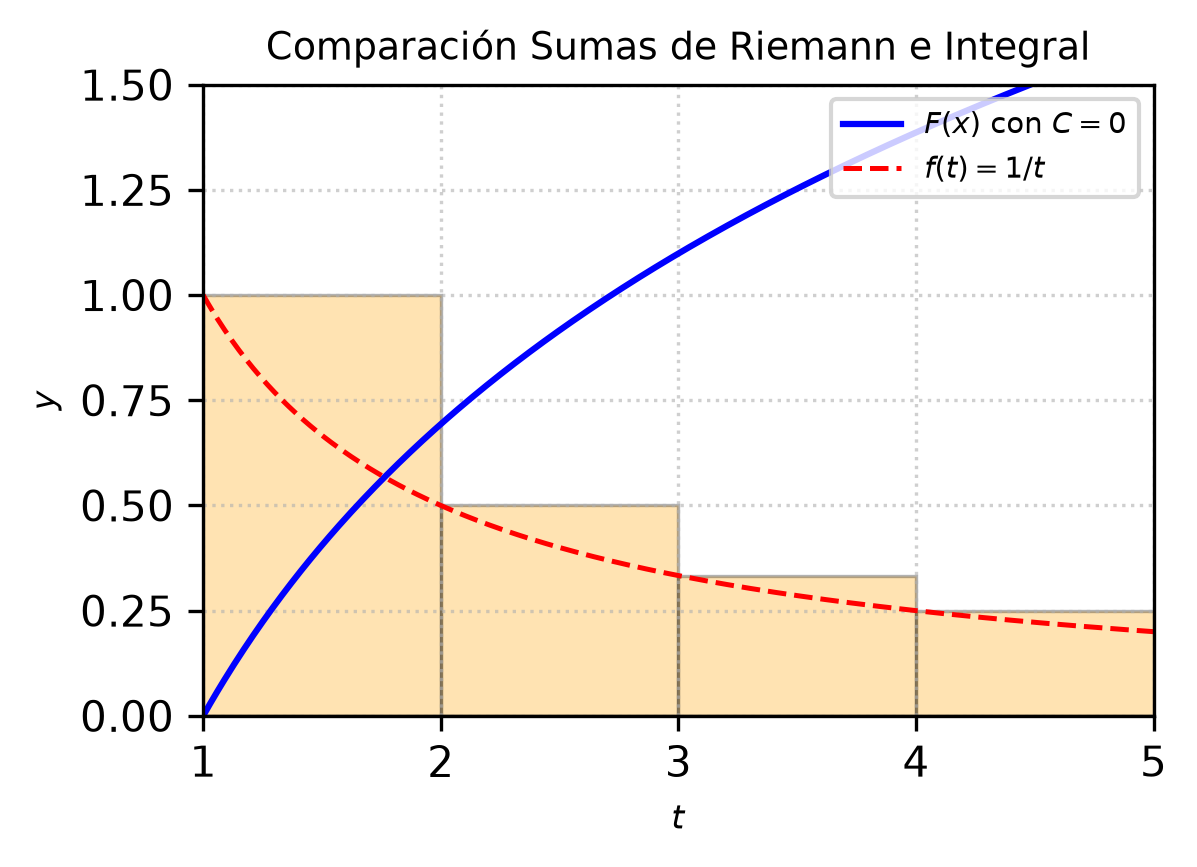
\includegraphics[width=\columnwidth]{semana_08/graficas/SEM08_P04_grafica.png}
	\caption{Representación gráfica de $f(x)$ y su antiderivada $F(x)$ evaluada para la constante de integración $C = 0$ (Problema 04).}
	\label{fig:problema04}
\end{figure}
